\documentclass[a4paper]{article} %style de document
\usepackage[utf8]{inputenc} %encodage des caractères
\usepackage[french]{babel} %paquet de langue français
\usepackage[T1]{fontenc} %encodage de la police
\usepackage[top=2cm,bottom=2cm,left=2cm,right=2cm]{geometry} %marges
\usepackage{graphicx} %affichage des images
\usepackage{hyperref}%rend actif liens et références
\usepackage{verbatim}%permet insertion de texte brut (du style le logo Latex)
%\usepackage{amssymb} %collection de symboles
\usepackage[dvipsnames]{xcolor}%importe les couleurs, l'option permet d'avoir encore plus de couleurs
\usepackage{sectsty}%permet de changer les couleurs des sections/titres, etc
\usepackage{tikz}%pour faire des figures
\usepackage{appendix} % Pour l'annexe
\usepackage[linesnumbered,ruled, french,onelanguage]{algorithm2e}

\begin{document}
\makeatletter
  \begin{titlepage}
  \centering
      {\large \textsc{Université de Caen Normandie}}\\
      \textsc{Licence informatique 2\up{ème} année}\\
    \vspace{1cm}
      
\includegraphics[width=0.25\textwidth]{images/unicaen.jpg}\\
    \vspace{1cm}
      {\large\textbf{	\@date\\
       Rapport Conception logicielle avancée}}\\
    \vfill
       {\LARGE \textbf{
       Solveur de Ricochet Robot}}\\
    \vspace{2em}
        {\large Lefevre Alex \& Malbec Elie \& Kablan Yoann \& Vouvou Brandon} \\
    \vfill
       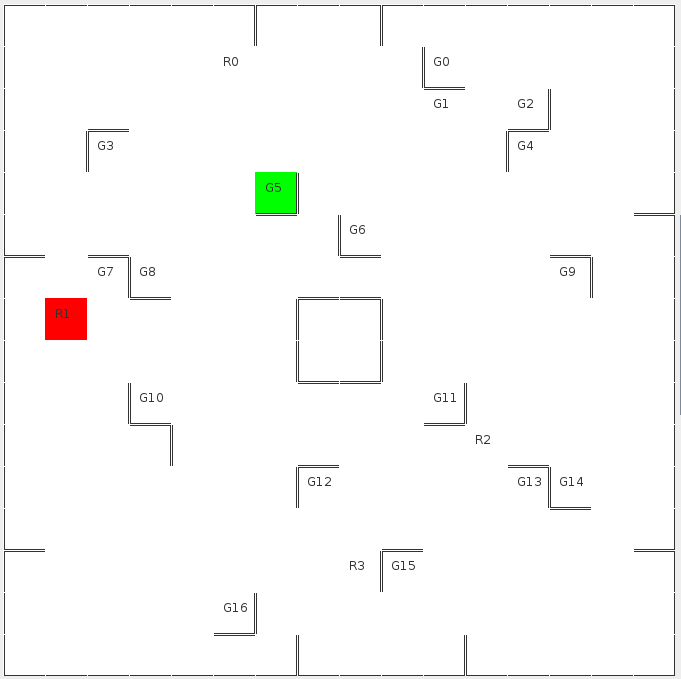
\includegraphics[height=0.4\textheight]{images/visuBoard.png}
     \vfill
  \end{titlepage}
\makeatother
\newpage
\tableofcontents
\newpage

\section{Introduction}
	\subsection{Introduction}
Dans le cadre de l'unité d'enseignement Conception Logicielle Avancée enseignée à l'Université de Caen en 2\up{ème} année de licence d'informatique, nous avons réalisé un solveur du jeu Ricochet Robot en Java. Nous avons formé un groupe de quatre étudiants : Alex Lefevre, Elie Malbec, Yoann Kablan et Brandon Vouvou pour concevoir une IA (intelligence artificielle) résolvant le jeu. Dans ce rapport, nous vous exposons les démarches qui nous ont permis de concevoir un algorithme de résolution ainsi que les difficultés rencontrées durant son élaboration.

Notre réflexion portée sur le concept du jeu et sa méthode de résolution nous ont motivés pour sélectionner ce projet parmi les autres.

	\subsection{Le jeu de Ricochet Robot}
	%expliciter les règles/but du jeu
Le jeu de Ricochet Robot est un jeu de société qui se joue sur un plateau. Ce plateau se compose de murs, d'objectifs et de robots. Le but est de déplacer les robots jusqu'à ce que l'un d'eux, le robot principal, arrive sur la case objectif sélectionnée. Les robots ne se déplacent qu'en ligne droite et doivent s'arrêter lorsqu'ils rencontrent un autre robot ou un mur. Le but est donc d'arriver sur la case cible tout en faisant le moins de mouvements possibles.
		%Le plateau
		%les murs
		%les robots
		%les objectifs/cibles
			\subsubsection{Le plateau}
Ricochet Robot est dans sa version originale un jeu de plateau composé d'une grille de taille $16*16$. Chacune des 256 cases est représentée par une paire de coordonnées $(x,y)$. Une case peut comporter des murs à gauche, à droite, en haut et en bas faisant office d'obstacle de déplacement aux quatre entités appelées \textit{robots}. La grille est délimitée par une bordure de murs extérieurs. Les murs sont appelés suivant leur direction : murs 'nord', 'sud', 'est' et 'ouest'. Quatre cases au centre du jeu forment une zone noire et ne sont pas accessibles car elles disposent de murs dans les quatre directions cardinales.

			\subsubsection{Les robots}
Les robots sont des entités placées aléatoirement sur le plateau du jeu. Deux robots ne peuvent pas être présents sur la même case au même moment ni dans les cases centrales. Chaque robot peut se déplacer suivant les directions cardinales jusqu'à ce qu'il rencontre un obstacle, ce dernier peut être de deux types : un mur ou un autre robot. Par exemple, pour un robot placé sur une case, il lui est impossible de se déplacer sur la droite si la case sur laquelle il est possède un mur à l'Est ou s'il y a un robot sur la case de droite adjacente. 

			\subsubsection{Les cibles}
De multiples cibles sont également placées dans les angles formés par deux murs. Un des robots dit robot principal doit atteindre la cible principale pour terminer le jeu. Les mouvements des robots annexes peuvent servir au robot principal pour créer de nouveaux obstacles de déplacement. Le but est de se rendre sur la cible principale avec le moins de mouvements possible.
Il y a 17 cibles sur le plateau, donc 17 tours de jeu dans le jeu original, cependant, dans notre cas, nous n'avons pas mis en place ces règles de jeu mais uniquement la méthode de résolution et la possibilité de jouer en interface graphique.%utilité de dire qu'on a pas fait un truc ?

			\subsubsection{Les positions dans le plateau}
Chaque position sur le jeu peut être représentée par des coordonnées sur un plan deux dimensions. Voici les positions utilisées, elles correspondent à l'indexation des objets avec la structure de tableau à double dimension. Comme nous pouvons le voir case $(0,0)$ est en haut à gauche.%et non en bas à gauche comme sur un grpahique par exemple.
\pagebreak

\begin{figure}[htpb]
\centering
  \begin{tikzpicture}[scale=0.4]
  \draw[step=1cm,gray,very thin] (0,0) grid (16,16); 
  \draw[ultra thick,->] (0,16) -- (0,0);
  \draw[ultra thick,->] (0,16) -- (16,16);
  \draw[thick] (0,0) -- (16,0);
  \draw[thick] (16,0) -- (16,16);
  \fill (7,7) rectangle (9,9);
  \foreach \k in {15,14,...,0}
  	{\node at (-0.8,15-\k+0.5) {\k};}
  \foreach \k in {0,1,...,15}
  	{\node at (\k+0.5,16.8) {\k};}
  \end{tikzpicture}
  \caption{Coordonnées sur le plateau de jeu}
\end{figure}

	\subsection{Objectif du solveur}
L'objectif de la résolution du jeu est de minimiser le nombre de déplacements nécessaires pour permettre au robot principal de se rendre sur l'objectif. Plusieurs solutions permettent d'arriver au résultat mais certaines sont plus rapides.

Chaque robot déplacé compte pour un mouvement. Le fait de changer la position de robots annexes apporte de nouvelles possibilités de déplacement. Nous avons développés deux manières de résoudre ce problème, chaque méthode comporte des avantages et des inconvénients que nous détaillerons par la suite. La complexité du problème réside dans le nombre de déplacements possible à chaque état de jeu. Un nombre exponentielle de d'états s'ajoutent à chaque mouvement.

\section{Développement du moteur de jeu}
La première étape pour la réalisation de ce projet était de concevoir le modèle du jeu. Pour cela, un premier package \texttt{modele} comporte l'ensemble des classes nécessaires à sa modélisation.

	\subsection{Plateau du jeu}
Pour modéliser le plateau, nous avons développé une classe \texttt{Board}. Cette dernière est constituée de 256 cases et représente l'état actuel du jeu. Les entités sont représentées par des classes \texttt{Robot} et \texttt{Goal}. Les robots et cibles ne sont pas directement placés sur le plateau mais possèdent leur propre position. Cela permet de ne pas vérifier dans chaque case la présence de telle ou telle entité.

Les robots et les cibles sont stockés dans des listes avec la structure de donnée \texttt{ArrayList}. Des références au robot principal et à la cible principale permettent de les distinguer des autres.

La construction du plateau de jeu est basée sur un fichier texte, ce fichier contient des coordonnées et une description des murs et des entités présentes (\ref{structFichier}). Cette construction est par défaut basée sur celle du plateau de jeu officiel. Mais il est possible de générer un plateau aléatoirement ou de choisir un autre fichier de configuration.

Voici le diagramme de classe donnant les principales méthodes utilisées sur le plateau mais également la structure des robots et cibles.
\pagebreak
\begin{figure}[!h]
	\begin{center}
	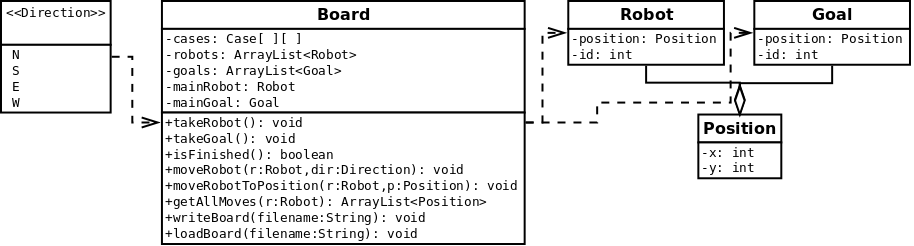
\includegraphics[scale=0.5]{./images/boardwithentities.png}
	\caption{Diagramme de classe du Board et des entités}
	\end{center}
\end{figure}

Le plateau dispose de méthodes qui lui permettent de bouger les robots, de tester si le jeu est terminé mais aussi de tirer une nouvelle cible ou un nouveau robot aléatoirement. Les directions sont listées depuis une énumération et les positions représentées avec deux coordonnées pour un plan deux dimensions.

Nous pouvons également remarquer que les 256 cases sont des objets \texttt{Case} stockées dans un double tableau. Cela permet un accès direct aux données mais aussi un parcours simplifié avec une largeur et une hauteur connue. La composition d'une case est la suivante :
\begin{figure}[htpb]
	\begin{center}
	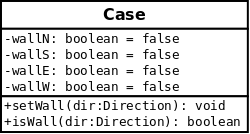
\includegraphics[scale=0.5]{./images/casediag.png}
	\caption{Classe Case}
	\end{center}
\end{figure}

Les quatre murs possibles sont par défaut désactivés puis activés avec la méthode \texttt{setWall} dans la direction donnée. Une fois les murs mis en place, ils ne changent plus durant la partie.%activé, désactivé, plus clair

	\subsection{Déplacements}
Concernant les déplacements, les méthodes \texttt{moveRobot} et \texttt{getAllMoves} nécessitent des tests supplémentaires. Il faut vérifier que les déplacement sont valides et donner les positions d'arrivées quand un obstacle est rencontré. Pour cela, des méthodes ont été implémentées dans la classe \texttt{Board} dont voici le diagramme :

\begin{figure}[htpb]
	\begin{center}
	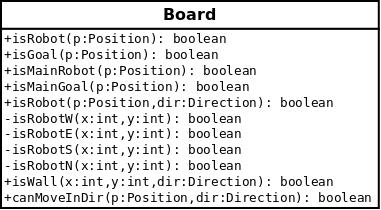
\includegraphics[scale=0.5]{./images/boardMove.png}
	\caption{Méthodes pour déplacements dans Board}
	\end{center}
\end{figure}

Les déplacements sont ainsi possibles en donnant spécifiant un robot et une direction à la méthode \texttt{moveRobot}. La position d'arrivée est renvoyée et le déplacement est effectué en mettant à jour la position du robot concerné. Notons également qu'une cible ne constitue pas un obstacle à un mouvement.

	\subsection{Visualisation du jeu}
Pour permettre de jouer au clavier et rendre le jeu plus visuel, une interface graphique à été développée en suivant le schéma MVC (Modèle Vue Contrôleur). Les murs sont représentés par des traits et les entités sont placées par rapport à leurs coordonnées respectives. Le robot en cours de déplacement est coloré en rouge et la cible principale en vert. Cette visualisation permet de mieux voir les données comparativement à une lecture sous forme textuelle.
La figure \ref{visuBoard} donne un aperçu de la vue sur le \texttt{Board}.

\begin{figure}[htpb]
	\begin{center}
	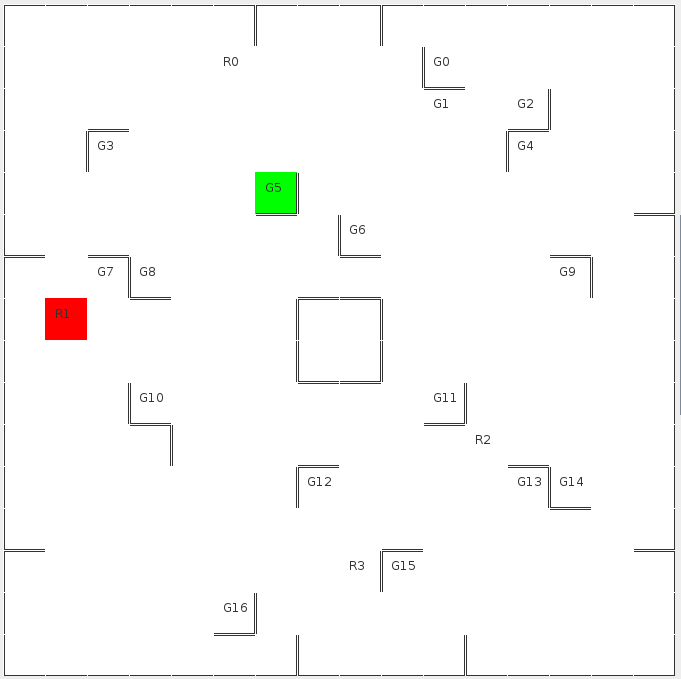
\includegraphics[scale=0.4]{./images/visuBoard.png}
	\caption{Visualisation graphique du jeu}\label{visuBoard}
	\end{center}
\end{figure}

	\subsection{Détails de l'implémentation}
Lors du développement de ce modèle de jeu, nous avons eu des difficultés quand aux structures de données à utiliser. L'utilisation du gestionnaire de version Git nous à permit de créer plusieurs versions plus ou moins stables du modèle. Dans un premier temps, nous avions décidé de placer les entités directement dans les cases du plateau de jeu. Cette méthode était très difficile à maintenir car les positions des entités étaient stockées dans des \texttt{HashMap}.

Nous avons par la suite abandonné ce système pour réaliser une seconde implémentation du modèle. Dans cette dernière, nous avons gardés la structure des cases, c'est à dire quatre attributs correspondants au murs possibles. Un ensemble de méthode ont été créées pour générer des plateaux aléatoires. C'est sur cette version que sera basée la prochaine utilisant les algorithmes de résolution.

\section{Méthodes de résolution}
	Dans cette partie, nous allons voir les deux algorithmes utilisés pour la résolution du jeu. Il s'agit de l'algorithme \textsl{A*} et de \textsl{BFS} (Breadth First Search). Chaque méthode possède des avantages et des inconvénients que nous allons détailler ci-dessous.
	
	\subsection{Historique du projet}
Durant le développement du projet, nous nous sommes tout d'abord penchés sur l'algorithme de résolution \textsl{A*}. Ce dernier possède un avantage théorique car il limite le nombre d'état possible grâce à une heuristique de plateau. L'implémentation de \textsl{A*} a nécessité l'utilisation de méthodes définies dans la classe \texttt{Board}. Cependant nous avons eu beaucoup de mal à trouver une heuristique cohérente permettant de trouver la solution. Après certaines recherches, nous avons décidés de se pencher sur l'algorithme \textsl{BFS}, ce dernier néglige la mémoire au profit de trouver une solution rapide. C'est cette méthode qui nous à donné le plus de résultats cohérents.

Pour mettre en place ces résolutions, une dernière version du modèle à été mise en place, avec des entités robots et cibles qui possèdent leur propre position. Cela permet de les déplacer virtuellement sur le jeu tout en ne stockant que ces positions pour les différents états.

	\subsection{Algorithme A*}
		\subsubsection{Principe}
L'algorithme \textsl{A*} est un algorithme de recherche de chemin dans un graphe entre un nœud initial et un nœud final. Dans notre cas, le nœud initial est l'état de base du plateau de jeu, les nœuds intermédiaires les possibles chemins empruntés par les robots et le nœud final l'état du jeu terminé.
Cet algorithme utilise une évaluation heuristique pour déterminer le meilleur chemin pour se rendre sur la cible.

Nous avons dû réaliser une structure de nœud avec une relation d'ordre suivant leur évaluation. En effet, l'évaluation d'un nœud $n$ est notée $f(n)$. La fonction d'évaluation $f(n)$ est un nombre réel positif ou nul, estimant le coût du meilleur chemin du nœud initial passant par n et arrivant au but. $f(n)$ se décompose en deux parties : $f(n) = g(n) + h(n)$
\begin{itemize}
\item $g(n)$ le coût du meilleur chemin ayant mené au nœud $n$ depuis le nœud initial.
\item $h(n)$ est une fonction d'estimation du coût restant entre un nœud $n$ d'un graphe et le but.
\end{itemize}

Ici $g(n)$ est définie par la somme des distances de Manhattan de la position du nœud $n$ à la cible $goal$. Cette somme défini le coût nécessaire pour se rendre à ce nœud depuis l'origine.
Pour $h(n)$, nous avons utilisé la distance de Manhattan du robot principal à la cible. Cette évaluation vaut 0 si le robot atteint la cible et est maximisée si le robot est loin de la cible.%dernière phrase mal dit

\textsl{A*} est optimal si l'heuristique $h(n)$ ne surestime jamais le coût pour se rendre au nœud suivant $n'$ et si les nœuds enfants possèdent une heuristique plus basse que celle du nœud courant.

Cet algorithme à besoin d'une liste dite $open$ qui contient les nœuds pas encore traités : i.e. la frontière de la partie du graphe explorée jusqu'à maintenant. Les nœuds sont triées selon l'estimé $f(n)$ la fonction d'évaluation. On explore les nœuds les plus prometteurs en premier. Et d'une liste dite $closed$ qui contient les nœuds déjà traités, i.e. à l'intérieur de la frontière délimitée par $open$.

	\subsubsection{Implémentation}
Pour implémenter cet algorithme, nous avons créer une classe \texttt{Solver} suivant un état du jeu donné. Les nœuds implémentent l'interface \texttt{Comparable} permettant d'établir une relation d'ordre entre eux. Les listes $open$ et $closed$ sont des \texttt{ArrayList<Node>}. Chaque nœud contient une position du robot principal.
Le diagramme de classe associé est la figure \ref{solverDiag};

\begin{figure}[htpb]
	\begin{center}
	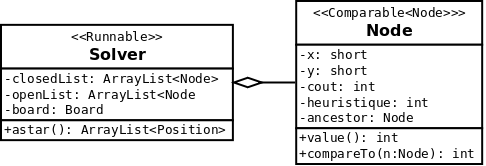
\includegraphics[scale=0.4]{./images/solver.png}
	\caption{Diagramme de la classe Solver}\label{solverDiag}
	\end{center}
\end{figure}

En suivant l'exécution de cet algorithme, nous pouvons trouver une solution n'impliquant que le robot principal. Cette résolution fonctionne si le chemin pour se rendre à la cible est direct. Cependant cela ne garantie pas qu'il s'agit du chemin optimum (avec peu de coups).

Nous avons donc tentés d'ajouter les mouvements des autres robots dans la liste $open$ après chaque coup joué avec différentes heuristiques : 
\begin{itemize}
\item Distance de Manhattan entre le robot principal et la cible
\item Somme des distances de tous les robots à la cible
\item Distance de Manhattan minimum après tous les coups possibles pour le robot principal
\end{itemize} 
Mais aucuns ne permet de résoudre le jeu car des coups joués sont jugés bons par leur valeur mais en réalité bloquants, inutiles ou inverses.
Il est très difficile de donner un poids différent à chaque état de jeu. Ce constat s'est confirmé par plusieurs rapports qui estiment que chaque mouvement (et donc chaque lien dans l'arbre) à un poids équivalent si c'est un robot annexe qui est déplacé.
Dans ce cas précis, la distance entre le robot principal et la cible principale ne change pas, tous les nœuds auront la même valeur, l'algorithme en choisira un au hasard et le jouera. Mais ce ne sera pas forcement un coup utile à la résolution.

Ce type d'algorithme n'est pas performant pour ce jeu, les déplacements sont effectués dans des directions et peuvent éloigner le robot pour qu'au coup suivant il atteigne sa cible. Toute la difficulté réside dans la création d'une heuristique complexe faisant intervenir des état futurs.

Nous avons en conséquence réalisé un \textsl{A*} déplaçant uniquement le robot principal.

		\subsubsection{Remarques}
L'algorithme \textsl{A*} permet de résoudre rapidement un chemin direct pour se rendre sur la cible. Mais dans la plupart des cas, ce chemin n'existe pas et le déplacement de robots secondaires est nécessaires. Il n'y a donc aucune garantie quand au résultat. De plus, le chemin peut contenir plus de mouvements que nécessaire, ne donnant pas pleine satisfaction par rapport au but de notre projet.

	\subsection{Algorithme BFS (Breadth First Search)}
		\subsubsection{Principe}	
Dans une recherche en largeur, il faut commencer à la racine $root$ qui est l'état initial. Puis ajouter tous les enfants $child$ de $root$ dans une liste depuis les mouvements possible. Pour chaque état $child$, pris l'un après l'autre, nous testons si c'est un état final, i.e. un jeu terminé dans notre cas avec le robot sur sa cible. Si aucun état final n'est rencontré dans tous les état $child$, génération de tous les états de niveau 2 à partir de chaque $child$. Une nouvelle liste d'état de niveau 2 est testée et ainsi de suite.

Si un état final est rencontré, remonter le chemin jusqu'à la racine $root$.

Cette méthode de résolution garantie un résultat rapidement, mais au détriment de la mémoire. De plus, la première solution est garantie d'être la solution optimum.

Le nombre d'état est exponentiel, ce que pose des problèmes de mémoire et empêche la résolution de long chemins. À l'état initial, il y a 4 robots qui peuvent se déplacer dans 4 directions, cela apporte 16 possibilités. Puis en profondeur 2, pour chacun des 16 cas, il y a 2 à 3 mouvements possibles pour chaque robot. L'algorithme est optimisé pour éviter les mouvements inverses. Certaines études montrent également qui pour de longs chemin, le fait de jouer en premier le robot principal donne plus de chance de trouver le chemin rapidement.

		\subsubsection{Implémentation}
Ricochet Robot est un problème complexe à résoudre, le nombre de cas augmente très rapidement dès la profondeur 6. Nous avons choisi de choisir ce algorithme car il permet de résoudre plus de situations de jeu. Mais les performances de notre modèle nous empêchent de trouver des chemins de plus de 6 mouvements en raison de manque de mémoire et d'optimisations. Chaque état est stocké suivant la classe interne \texttt{State} contenue dans la classe \texttt{BFSSearch}, figure \ref{bfs}.

\begin{figure}[htpb]
	\begin{center}
	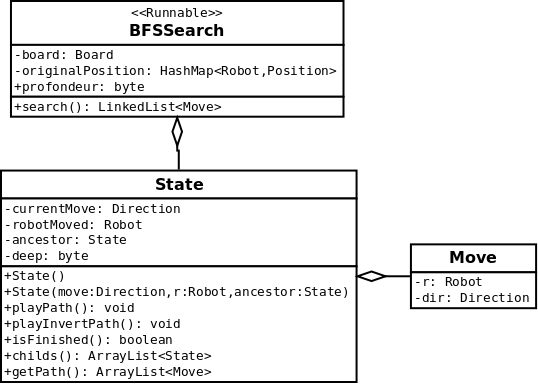
\includegraphics[scale=0.3]{./images/bfssearch.png}
	\caption{Diagramme de classe BFSSearch}\label{bfs}
	\end{center}
\end{figure}

Ainsi, la mémoire utilisée pour stocker un état de jeu est assez faible, un lien avec tous les ancêtres depuis l'état courant permet de tracer le chemin parcouru par tous les robots depuis le plateau de base contenu dans la classe \texttt{BFSSearch}. Pour savoir si l'état est considéré comme terminé, il faut reconstituer le chemin depuis l'origine, puis jouer chaque coup depuis le plateau de base. Ensuite vérifier si le robot est sur la cible, enfin reconstituer le plateau de base en réinitialisant les positions des robots depuis \texttt{originalPosition}.

Pour gagner du temps lors de l’exécution il serait possible de déterminer les positions d'arrivée à chaque état et de placer directement le robot à cet endroit à la place de réaliser les multiples tests de déplacement.

Le temps nécessaire pour trouver un chemin est assez court pour des résolutions en 6 mouvements, mais au delà il faut une puissance de calcul supplémentaire et de la mémoire. En effet, chaque état de chaque profondeur est stocké en mémoire, une optimisation viserait à supprimer ces états et les retrouver en chemin inverse.

		\subsubsection{Détails}
Le pseudo-code de l'algorithme BFS est l'algorithme \ref{algobfs}.

\begin{algorithm}
\DontPrintSemicolon
\SetAlgoVlined
\KwIn{Plateau initial $Board$ $b$}
\KwOut{Liste chaînée de $Move$ pour la résolution}
$Bool$  $finished \gets false$\;
$State$  $root \gets b$\;
$Add$ $root$ to $nodes$ $list$\; 
\While{$finished=false$} {
	new $list$ $childs$\;
	\For{State s in nodes}{
	add all $childs(s)$ to $childs$ $list$\;
	}
	\For{State s in childs}{
		\If{$isFinished(s)$}{
			\Return{$path(s)$}
		}
	}
	$nodes \gets childs$\;
}
\Return{$null$}\;
\caption{{\sc Search} Algorithme BFS de résolution}
\label{algobfs}
\end{algorithm}

	\subsection{Conclusion}
Nous avons eu l'occasion d'implémenter deux algorithmes de recherche. L'un d'eux, \textsl{A*} n'est pas une solution viable sans une heuristique complexe utilisant les états futurs. Mais cette méthode à l'avantage d'être très rapide en explorant uniquement les cas jugés utiles. Nous n'avons pas réussi à déterminer cette heuristique. De plus, le chemin trouvé n'est pas forcement le chemin optimal.

Le second algorithme nous a cependant permis de résoudre une partie du problème, des améliorations pourraient lui être apportées pour explorer des chemins plus complexes et coûteux en mémoire. Cette méthode à l'avantage de trouver la bonne solution la plus rapide pour arriver au but. Sa complexité est exponentielle et son temps d'exécution assez rapide car la majorité des solutions se trouvent en moins de 6 déplacements.

Pour ouvrir sur d'autres possibilités, l'algorithme DFS (Deep First Searching) est une exploration en profondeur qui nécessite peu de mémoire au détriment du temps de résolution. Les branches sont explorées jusqu'au dernier nœud possible (avant de faire des mouvements arrières).

\section{Fonctionnalités implémentées et architecture}
	\subsection{Interface graphique}
	Une interface graphique\up{\ref{interface}} permet de visualiser l'état d'un plateau de jeu. Le choix de la cible s'effectue via une liste déroulante, de même pour le robot colorié en rouge. Il est possible de déplacer le robot en cours dans la direction souhaitée par l'appui sur les flèches directionnelles.
	Chaque action entraîne la mise à jour de l'interface graphique conformément à la structure MVC. Un message s'affiche lors de la résolution du jeu.
	Des boutons permettent de lancer les algorithmes de recherche pour trouver une solution au problème actuel. C'est à dire pour permettre au robot de se rendre sur la cible.
	La remise à zéro du plateau est un rechargement du fichier de configuration du jeu officiel.

\begin{figure}[htpb]
	\begin{center}
	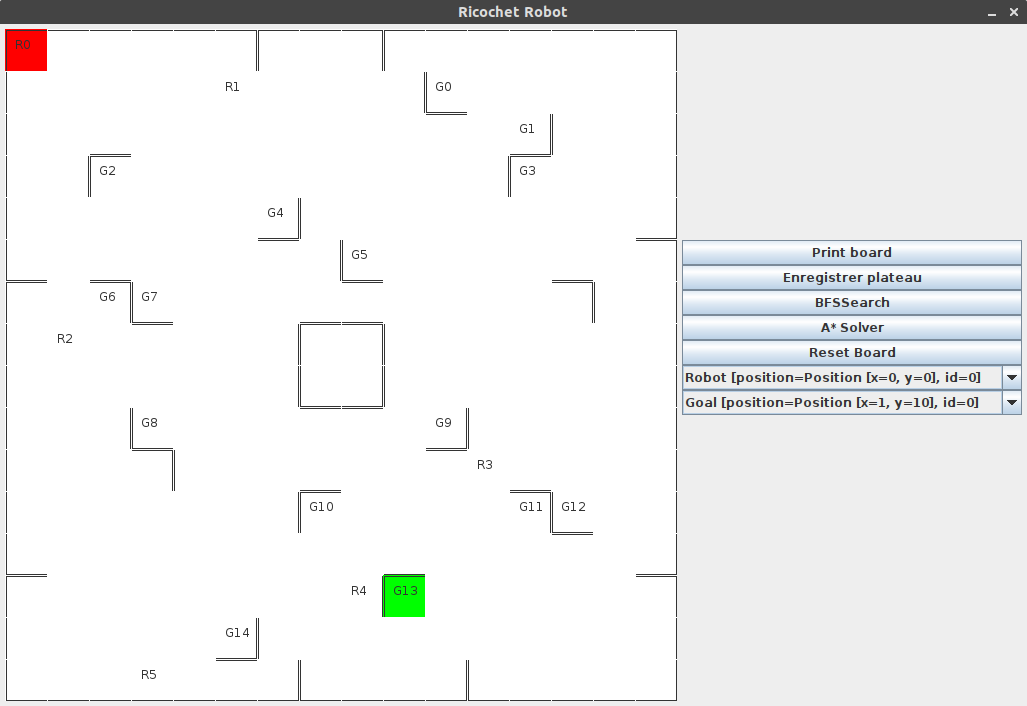
\includegraphics[scale=0.4]{./images/interface.png}
	\caption{Interface de jeu}\label{interface}
	\end{center}
\end{figure}

	\subsection{Génération aléatoire de plateau}
La génération aléatoire de plateau créé un fichier qui pourra être chargé comme plateau de jeu. Sa génération repose sur certaines règles :
\begin{itemize}
\item Création d'un bordure extérieure du jeu.
\item Création d'un mur sur chaque coté de chaque quart de terrain.
\item Quatre cases centrales inaccessibles.
\item Création de 17 angles formés par des murs, ne devant ni toucher les cases centrales, ni les bordures extérieures, ni d'autres angles. Il y a 4 angles par quart de terrain et 1 autre placé aléatoirement.
\item Placement des cibles dans les angles
\item Placement aléatoire de 4 robots, jamais dans la même case.
\end{itemize}

Il est également possible d'enregistrer le plateau courant depuis l'interface graphique pour reprendre une configuration et de le recharger par la suite.

		\subsubsection{Format du fichier de configuration}\label{structFichier}
Le fichier contenant les données de configuration d'un plateau de jeu est composé de la manière suivante :
\begin{enumerate}
\item Coordonnée x de la case
\item Coordonnée y de la case
\item Description de la case avec des espaces entre chaque caractéristique :
\begin{itemize}
\item N S E W pour les murs
\item R G pour les robots et cibles
\end{itemize}
\end{enumerate}
Par exemple, \textsl{0 0 W N R} donne pour la case en position $(0,0)$ un mur à l'Ouest, un mur au Nord et un Robot.

Il est possible d'ajouter d'autres robots et de nouvelles cibles en ajoutant de nouvelles lignes de configuration. Elles peuvent être mélangées.

	\subsection{Architecture du projet}
Voici l'architecture de notre projet :

\makeatletter
\newcount\dirtree@lvl
\newcount\dirtree@plvl
\newcount\dirtree@clvl
\def\dirtree@growth{%
  \ifnum\tikznumberofcurrentchild=1\relax
  \global\advance\dirtree@plvl by 1
  \expandafter\xdef\csname dirtree@p@\the\dirtree@plvl\endcsname{\the\dirtree@lvl}
  \fi
  \global\advance\dirtree@lvl by 1\relax
  \dirtree@clvl=\dirtree@lvl
  \advance\dirtree@clvl by -\csname dirtree@p@\the\dirtree@plvl\endcsname
  \pgf@xa=0,5cm\relax
  \pgf@ya=-0,45cm\relax
  \pgf@ya=\dirtree@clvl\pgf@ya
  \pgftransformshift{\pgfqpoint{\the\pgf@xa}{\the\pgf@ya}}%
  \ifnum\tikznumberofcurrentchild=\tikznumberofchildren
  \global\advance\dirtree@plvl by -1
  \fi
}

\tikzset{
  dirtree/.style={
    growth function=\dirtree@growth,
    every node/.style={anchor=north},
    every child node/.style={anchor=west},
    edge from parent path={(\tikzparentnode\tikzparentanchor) |- (\tikzchildnode\tikzchildanchor)}
  }
}

\begin{figure}[h]
\begin{center}
\begin{tikzpicture}[dirtree,scale=0.7]
 	    
\node {src} 
    child { node {ricochet }
    	child { node {gui} 
    		child { node {RicochetGUI.java
			} }
    		child { node {Start.java
			} }
   			child { node {VueBoard.java
			} }
			child { node {VueCase.java
			} }
			child { node {VueMenu.java
			} }
    }
    	child { node {modele}    		 
    		child { node {Board.java
			} }
    		child { node {Case.java
			} }
   			child { node {Direction.java
			} }
			child { node {Goal.java
			} }
			child { node {Position.java
			} }
			child { node {Robot.java
			} }
			child { node {Solver.java
			} }
			child { node {Start.java
			} }
			child { node {BFSSearch.java
			} }
    }
    	child { node {util} 		 
    		child { node {AbstractModeleEcoutable.java
			} }
    		child { node { EcouteurModele.java
			} }
   			child { node {ModeleEcoutable.java
			} }
   	}
   		child { node {dist}    		 
    		child { node {board.txt
			} }
    }}    	       	     
    ;   
\end{tikzpicture}
\end{center}
\caption{Arborescence des dossiers}
\end{figure}
\pagebreak

\section{Expérimentations}
	\subsection{Comparaison du temps de calcul}
	
	
Dans le cas de notre jeu la complexité a été très variable, ce qui est la cause du nombre d'information a traiter et aussi aux algorithmes de recherche.En effet  la complexité est un domaine de l'informatique qui étudie la quantité de ressources (temps, espace mémoire, etc.) dont a besoin un algorithme pour résoudre un problème algorithmique.Ici nous comparons a travers une courbe le temps que met les deux algorithmes a trouver la solution du jeu en fonction du nombre de mouvement a effectuer.	
	\begin{figure}[h]
	\begin{center}
	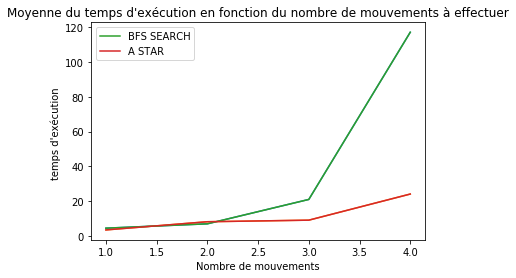
\includegraphics[scale=0.37]{./images/time.png}
	\caption{Courbes du temps d’exécution des algorithmes  en fonction du  nombre de mouvements pour les Algorithmes A* et BFS}
	\end{center}
\end{figure}
\newline
Au vu de cela nous pouvons noter que cette différence de temps d’exécution entre les deux algorithmes est en parti dû  à la différence du  nombres de nœuds explorés, et aux différences fondamentales des deux algorithmes.

	
	\subsection{Nombre de nœuds explorés}
On a ici la courbe représentant le nombre de nœuds explorés en fonction du nombre de mouvements effectués dans l'algorithme \textsl{BFS}. On observe a travers ces figures une évolution de façon exponentielle des valeurs des nœuds parcourus lors de la recherche de solution au cours de l’exécution de l'algorithme \textsl{BFS}. Le tableau suivant représente le nombre de nœuds moyens parcourus en fonction du nombre de mouvements des résolutions.En ce qui concerne l'algorithme A* on observe un très faible nombre de nœuds explorés par rapport aux nœuds explorés lors de l’exécution de l'algorithme \textsl{BFS} , ce qui est en effet dû a la différence de paramètres pris en compte , et donc à la différence qu'oppose ces deux algorithmes dans la recherche de la solution au jeu. 

\begin{figure}[h]
	\begin{center}
	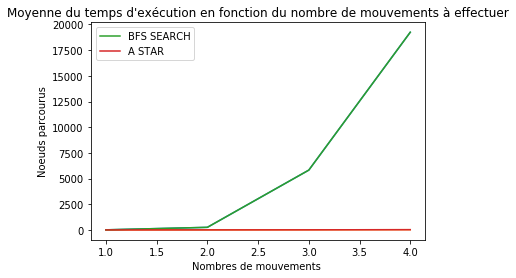
\includegraphics[scale=0.37]{./images/node.png}
	\caption{Courbes du nombre de nœuds en fonction du  nombre de mouvements pour les Algorithmes A* et BFS
	 }
	\end{center}
	\begin{center}
	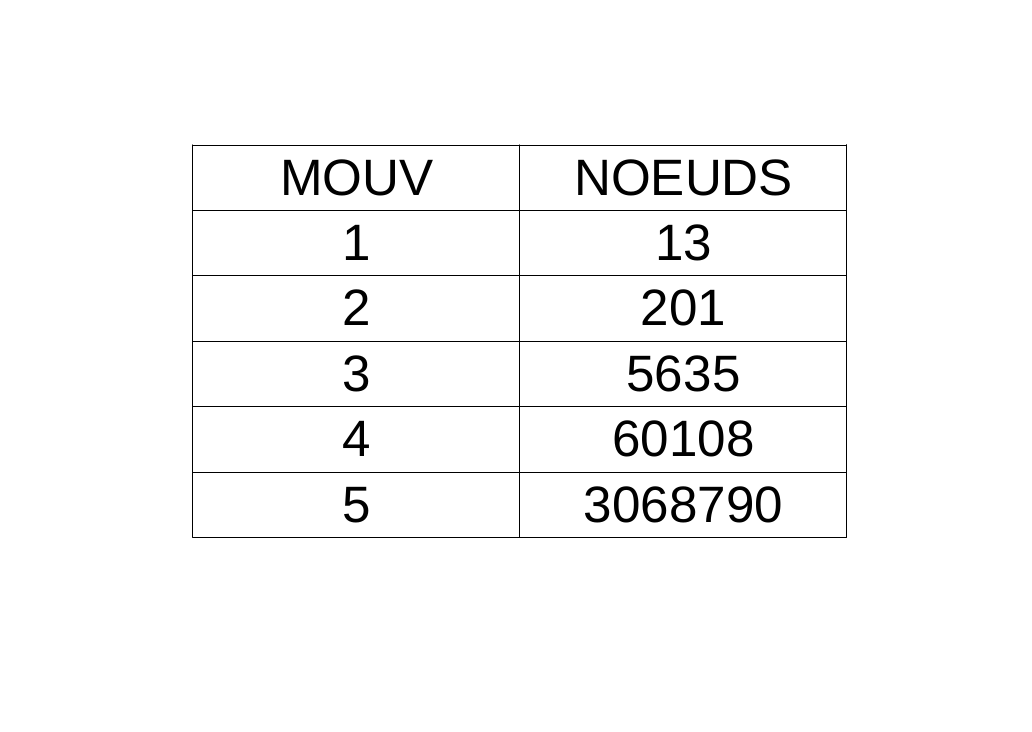
\includegraphics[scale=0.14]{./images/tabBFS.png}
	\caption{tableau du nombre de nœuds en fonction du  nombre de mouvements}
	\end{center}
\end{figure}


\section{Conclusion}
Ce projet à été très formateur pour l'ensemble du groupe, nous avons pu découvrir certaines pratiques algorithmiques intéressantes. La gestion du projet avec une succession de versions permet à chacun d'essayer certaines méthodes sans impacter le tronc commun. La question de l'heuristique dans des graphes est complexe et nécessite de l'expérience. De plus, ce projet est perfectible, par une série d'améliorations possible :
\begin{itemize}
\item Mise en place d'un timer de jeu pour limiter le temps de résolution à la fois pour un joueur humain et pour les algorithmes.
\item Ajout de scores pour un jeu multijoueur.
\item Réalisation d'un éditeur de plateau graphique.
\item Amélioration des algorithmes de recherche, notamment le BFS.
\item Sélection des cibles et robots au clic de la souris et amélioration de l'interface graphique.
\end{itemize}

\begin{thebibliography}{9}
\bibitem{ref1} Hugo Larochelle, chercheur en apprentissage automatique et chercheur chez Google Brain. \url{http://info.usherbrooke.ca/hlarochelle/cours/ift615_E2013/contenu.html}
\bibitem{ref2} Course:CPSC:Artificial Intelligence/States and Searching, The University of British Columbia \url{https://wiki.ubc.ca/Course:CPSC:Artificial_Intelligence/States_and_Searching}
\bibitem{ref3} A Case Study for Human Complex Problem Solving, 15 Septembre 2005
\bibitem{ref4} MoutainWest RubyConf 2015 - Solving Ricochet Robots \url{https://www.youtube.com/watch?v=fvuK0Us4xC4}
\bibitem{ref5} Wikipedia, Algorithme A* \url{https://fr.wikipedia.org/wiki/Algorithme_A*}
\bibitem{ref6} Wikipedia, Algorithme de parcours en largeur \url{https://fr.wikipedia.org/wiki/Algorithme_de_parcours_en_largeur}
\end{thebibliography}
\end{document} %fin du document

